\documentclass[a4paper, 10pt, final, garamond]{book}
\usepackage{cours-preambule}
\graphicspath{{./figures/}}

\makeatletter
\renewcommand{\@chapapp}{Contr\^ole de connaissances}
\makeatother

% \toggletrue{student}
% \toggletrue{corrige}
\renewcommand{\mycol}{black}

\begin{document}
\setcounter{chapter}{18}

\settype{enon}
\settype{solu}

\chapter{Forces intermoléculaires et moments\ifstudent{ (12')}}

\begin{enumerate}[label=\sqenumi]
	\nitem{4}%
	Identifier les substances possédant la température de fusion \textbf{la plus
		basse et la plus haute} parmi la liste suivante~: hélium \ce{He}, argon
	\ce{Ar}, méthane \ce{CH4}, acide éthanoïque \ce{CH3COOH}. Justifier de manière
	\textbf{précise et concise} (plus court qu'en TD) sans justifier l'ordre des
	températures de fusion intermédiaires.
	\smallbreak
	\psw{
		C'est l'hélium \pt{1} qui a la plus faible, étant donné qu'il correspond au
		plus petit corps pur stable et inerte, n'ayant aucune interaction de
		\textsc{VdW} \pt{1} notable. L'élément qui a la plus haute sera l'acide
		éthanoïque \pt{1}, étant donné sa capacité à créer des liaisons hydrogènes
		\pt{1} en sont sein (\ce{H} relié à \ce{O}).
	}
	\nitem{4}%
	Soit une force $\Ff$~: comment s'exprime son moment en O~? son moment par
	rapport à un axe orienté $\D$~? Démontrer alors \textbf{à l'aide d'un schéma}
	l'expression du moment $\Mc_{\D}(\Ff)$ utilisant le bras de levier pour une
	force $\Ff$ se décomposant en $\Ff_{\parr}$ et $\Ff_{\perp}$.
	\smallbreak
	\vspace{-15pt}
	\begin{isd}[interior hidden]
		\vspace{-15pt}
		\psw{
			\begin{DispWithArrows*}[fleqn, mathindent=0pt]
				\Mcf_{\Or}(\Ff) = \OM \wedge \Ff
				\quad & \stm[-1]{\text{et}} \quad
				\Mc_{\D}(\Ff) = (\OM \wedge \Ff)\cdot \ud
				\\\Ra
				\Mcf_{\rm O}(\Ff)
				& =
				\OM \wedge (\Ff_{\parr} + \Ff_{\perp})
				\\\Lra
				\Mcf_{\rm O}(\Ff)
				& =
				\underbracket[1pt]{\OM \wedge \Ff_{\parr}}_{\perp \ud} +
				\underbracket[1pt]{\OM \wedge \Ff_{\perp}}_{\parr \ud}
				\\\Ra
				\Mc_{\D}(\Ff)
				& \stm{=}
				0 +
				\left( \OMr \norm{\Ff_{\perp}}\sin(\a)\ud \right)\cdot \ud
				\\\Lra
				\Aboxed{\Mc_{\D}(\Ff)
					& \stm[-1]{=}
					\underbracket[1pt]{\OMr \sin(\a)}_{\pm d}\norm{\Ff_{\perp}}
				}
				\qed
			\end{DispWithArrows*}
		}
		\vspace{-15pt}
		\tcblower
		\begin{center}
			\sswitch{
				\includegraphics[width=.85\linewidth, draft=true]{bras_levier-dessus_complete}
			}{
				\includegraphics[width=.85\linewidth]{bras_levier-dessus_complete}
			}
			\vspace{-15pt}
			\captionof{figure}{Bras de levier (vue du dessus) \protect\pt{1}}
		\end{center}
	\end{isd}
	\nitem{6}%
	Démontrer le théorème du moment cinétique par rapport à un point O fixe.
	\smallbreak
	\begin{isd}
		\vspace{-15pt}
		\psw{
			\begin{DispWithArrows*}[fleqn, format=LrCl]
				\text{PFD~:}
				&
				\dv{\pf}{t}
				& \stm{=} &
				\sum_i\Ff_i
				\CArrow{$\OM \wedge \cdot $}
				\\\Ra
				&
				\OM\wedge\dv{\pf}{t}
				& \stm{=} &
				\OM\tikzmark{om}\wedge\sum_i\tikzmark{ff}\Ff_i
				\\\text{Or}
				&
				\dv{\Lcf_{\Or/\Rc}(\Mr)}{t}
				& \stm{=} &
				\dv{\tikzmark{dv}}{t}
				\left(\OM\tikzmark{omd}
				\wedge\pf\tikzmark{pfd}
				\right)
			\end{DispWithArrows*}
		}
		\vspace{-15pt}
		\tcblower
		\vspace{-15pt}
		\psw{
			\begin{align*}
				\Lra
				\dv{\Lcf_{\Or/\Rc}(\Mr)}{t}
				                            & =
				\underbracket[1pt]{
					\xunderbracket{\dv{\OM}{t}}_{\parr\vf}
					\stm(un){\wedge}
					\xunderbracket{\pf}_{\parr\vf}
				}_{=\of}
				+ \OM\wedge\dv{\pf}{t}
				\\
				\beforetext{Ainsi,}
				\dv{\Lcf_{\Or/\Rc}(\Mr)}{t} & \stm{=}
				\sum_i\OM\wedge\Ff_i \stm{=} \sum_i\Mcf_{\Or}(\Ff_i)
			\end{align*}
		}
		\tikz[remember picture, overlay]
		\draw[-stealth, transform canvas={yshift=12pt}, color=\sswitch{white}{black}]
		([shift={(-6pt,0)}]pic cs:om) to[out=90, in=90] (pic cs:ff)
		;
		\tikz[remember picture, overlay]
		\draw[-stealth, transform canvas={yshift=6pt}, color=\sswitch{white}{black}]
		(pic cs:dv) to[out=90, in=90] ([shift={(-6pt,6pt)}]pic cs:omd)
		;
		\tikz[remember picture, overlay]
		\draw[-stealth, transform canvas={yshift=6pt}, color=\sswitch{white}{black}]
		(pic cs:dv) to[out=90, in=90] ([shift={(-6pt,6pt)}]pic cs:pfd)
		;
		\vspace{-15pt}
	\end{isd}
	\nitem{8}%
	On étudie le mouvement d'une masse suspendue à un fil de longueur $\ell =
		\cte$ dans le référentiel du laboratoire supposée galiléen. Indiquer le repère
	choisi et le répérage qui en découle, faire un schéma puis déterminer
	l'équation du mouvement du pendule simple par le théorème du moment cinétique
	scalaire en utilisant le bras de levier.
	\smallbreak
	\noindent
	\begin{minipage}{0.70\linewidth}
		\psw{
			\begin{enumerate}[label=\arabic*)]
				\bitem{Repère}~: $(O,\ur,\ut,\uz)$ base cylindrique (voir schéma).
				\bitem{Repérage}~: $\OM = \ell\ur$, $\vf = \ell\tp\ut$. \pt{1}
				\bitem{BdF}~:
				\vspace{-15pt}
				\[
					\pt{1}
					\begin{array}{ll}
						\textbf{Poids}   & \Pf =
						m\gf =
						mg(\cos\th \ur - \sin\th \ut)  \\
						\textbf{Tension} & \Tf = -T\ur
					\end{array}
				\]
				\vspace{-10pt}
				\bitem{Calcul des moments}~:
				\[
					\left\{
					\begin{array}{rcl}
						\Mc_{z}(\Pf) & \stm[-1]{=} & - mg\,\ell \sin(\theta)
						\qar d = \ell \sin(\theta) \qet \text{sens horaire} \pt{1}
						\\
						\Mc_{z}(\Tf) & \stm[-1]{=} & 0
						\quad \quad \quad \quad \quad \qar \Tf \parr \OM
						\\
						\Lc_{z}(\Mr) & =           &
						\left((\ell\ur)\wedge(m\ell\tp\ut) \right)\cdot \uz \stm[-1]{=}
						m\ell^2\tp
					\end{array}
					\right.
				\]
				\bitem{TMC}~:
				\vspace{-25pt}
				\begin{align*}
					\dv{\Lc_z}{t}\/(\Mr) \stm{=} \Mc_z(\Pf)
					\Lra
					m\ell^2\tpp                          & = -mg\ell\sin\th + 0
					\\\Lra
					\Aboxed{\tpp + \frac{g}{\ell}\sin\th & = 0}
					\qed
				\end{align*}
			\end{enumerate}
		}
		\vspace{-15pt}
	\end{minipage}
	\hfill
	\begin{minipage}{0.25\linewidth}
		\begin{center}
			\sswitch{
				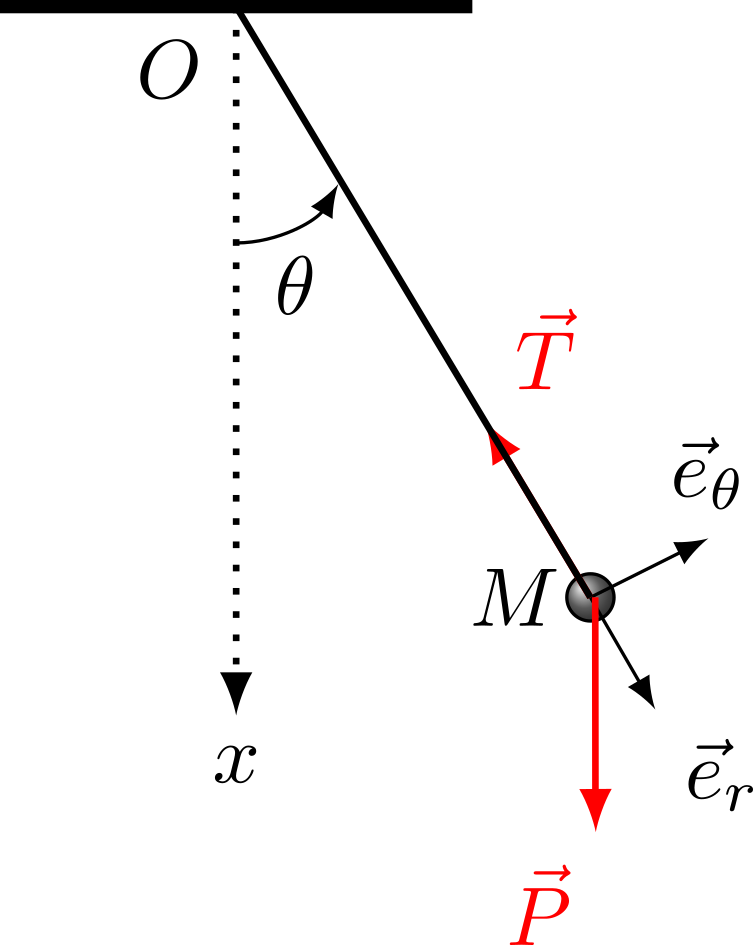
\includegraphics[width=\linewidth, draft=true]{pendule_plain}
			}{
				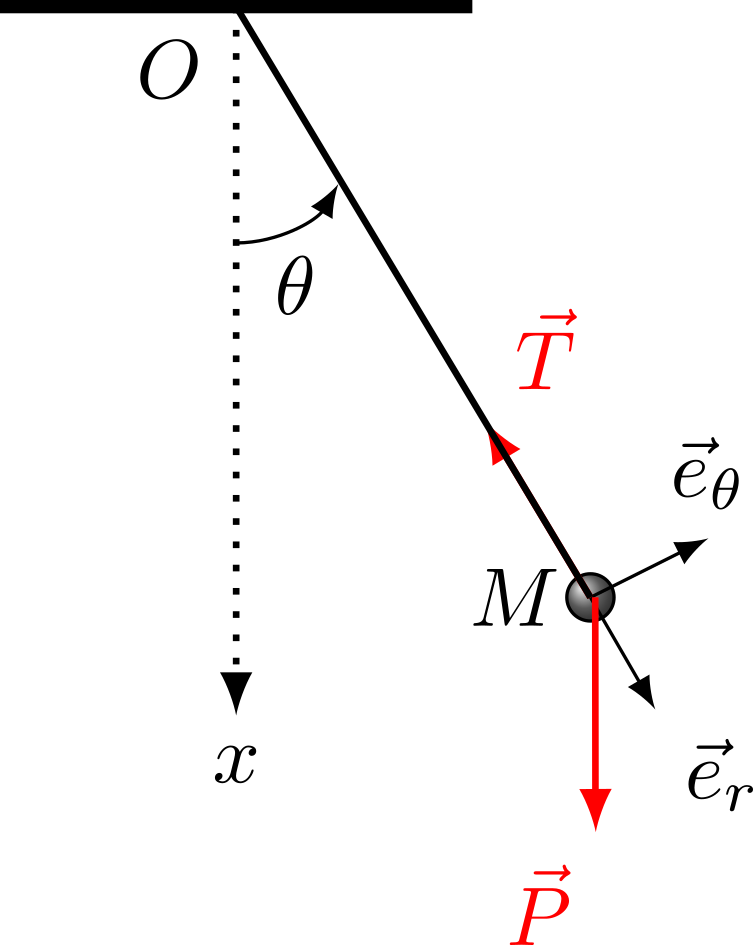
\includegraphics[width=\linewidth]{pendule_plain}
			}
			\captionsetup{justification=centering}
			\captionof{figure}{\\Pendule simple \protect\pt{1}}
		\end{center}
	\end{minipage}
	\ifstudent{
		\begin{tikzpicture}[remember picture, overlay]
			\node[anchor=north west, align=left]
			at ([shift={(1.4cm,0)}]current page.north west)
			{\\[5pt]\Large\bfseries Nom~:\\[10pt]\Large\bfseries Prénom~:};
			\node[anchor=north east, align=right]
			at ([shift={(-1.5cm,-17pt)}]current page.north east)
			{\Large\bfseries Note~:\hspace{1cm}/20};
		\end{tikzpicture}
	}
\end{enumerate}
\end{document}
